\documentclass{article}
\usepackage[margin=1.25in]{geometry}
\usepackage[utf8]{inputenc}
\usepackage{graphicx}
\usepackage[section]{placeins}
\usepackage{float}
\usepackage[italian]{babel}
\usepackage{hyperref}
%per il codice, usare:
%\usepackage{listings}

\title{Particles}
\author{Giulio Spadaro}
\date{November 2022}

\begin{document}
\maketitle

\section{Introduzione}
\label{Introduzione}
Lo scopo del programma prodotto è quello di generare su base casuale, sfruttando le librerie di PRNG di ROOT, un numero ben definito di eventi ed analizzare i risultati di tali eventi. In particolare, avviando il programma, vengono simulati \(10^5\) eventi ciascuno da \(100\) particelle di \(7\) tipi diversi, per un totale, dunque, di \(10^7\) particelle. Segue ad ogni evento, al fine di immagazzinare i dati ottenuti, una fase di riempimento di un certo numero di istogrammi, che fungono da base per la successiva analisi statistica dei risultati, riportata nella sezione \ref{Analisi dei risultati}. Inoltre, alcuni di questi istogrammi, nell'ottica di facilitare l'intepretazione dei dati, vengono rappresentati graficamente attraverso i metodi di disegno di ROOT, i cui prodotti finali possono sempre essere trovati nella sezione \ref{Analisi dei risultati}.
\section{Struttura del codice}
\label{Struttura del codice}
Il codice del programma è suddiviso in un totale di \(3\) header (\texttt{ParticleType.hpp}, \texttt{ResonanceType.hpp} e \texttt{Particle.hpp}) e \(5\) file sorgente, \(3\) dei quali (\texttt{ParticleType.cpp}, \texttt{ResonanceType.cpp} e \\ \texttt{Particle.cpp}) sono dedicati alla definizione dei metodi dichiarati nei corrispondenti file di intestazione; i restanti \(2\), tramite l'uso delle librerie di ROOT, contengono invece le istruzioni per la generazione casuale degli eventi e l'analisi dei dati da essa ottenuti (\texttt{Simulation.cpp} e \texttt{DataAnalysis.cpp}). In particolare:
\begin{itemize}
    \item In \texttt{ParticleType.hpp}, viene dichiarata la classe \texttt{ParticleType}, dotata di \(3\) dati privati,
    \begin{itemize}
        \item \texttt{char* const fName\_}, che descrive il nome della particella;
        \item \texttt{double const fMass\_}, che indica la massa della particella;
        \item \texttt{int const fCharge\_}, che indica la carica della particella.
    \end{itemize}
    Questi dati vengono poi inizializzati da un costruttore pubblico della classe e possono essere ottenuti dall'utente tramite i rispettivi getters pubblici (\texttt{char* GetfName() const}, \texttt{double GetfMass() const} e \texttt{int GetfCharge() const}), dichiarati in \texttt{ParticleType.hpp} e poi definiti in \texttt{ParticleType.cpp}. Inoltre, sono presenti altri due metodi pubblici virtuali, \texttt{virtual void Print()}, che produce una stampa a schermo dei valori dei dati privati, e \texttt{virtual double GetfWidth() const}, la cui utilità verrà chiarita nella trattazione della classe \texttt{ResonanceType}. Infatti, questi ultimi due metodi vengono ereditati dalla classe \texttt{ResonanceType}, dichiarata in \texttt{ResonanceType.hpp} e definita in \texttt{ResonanceType.cpp}.
    \item In \texttt{ResonanceType.hpp}, viene definita la classe \texttt{ResonanceType}, che eredita la parte pubblica di \texttt{ParticleType}, e vi viene aggiunta un attributo privato (\texttt{double const fWidth\_}) che consente di tenere conto della larghezza di risonanza delle particelle instabili della simulazione. Viene inoltre fatto l'override dei metodi pubblici \texttt{double GetfWidth() const} e \texttt{void Print()}, dove viene aggiunta la stampa a schermo della larghezza di risonanza oltre alle altre proprietà delle particelle. Vi è infine un costruttore pubblico. 
    \item \texttt{In Particle.hpp} viene poi dichiarata la classe \texttt{Particle} e i relativi metodi (definiti in \texttt{Particle.cpp}). Gli attributi privati di \texttt{Particle} sono:
    \begin{itemize}
        \item \texttt{std::vector\(<\)ParticleType *\(>\) static fParticleType}, un contenitore statico di puntatori a istanze di \texttt{ParticleType}, che consente di trattare  tutti i tipi di particelle semplicemente attraverso l'assegnamento (gestito dal costruttore e dal metodo privato \texttt{int static FindParticle(char)}) di un indice (\texttt{int fIndex}) ad ogni istanza di \texttt{Particle}. In questo modo, ogni volta che viene generata una particella, fatta sola eccezione delle componenti dell'impulso, relativi nome, massa e carica, vengono recuperati tramite il solo \texttt{fIndex}, risparmiando così notevolmente in overhead, attingendo la caratterizzazione della specie di ogni particella ad un numero estremamente limitato di elementi statici racchiusi in \texttt{fParticleType};
        \item \texttt{int static const fMaxNumParticleType}, ovvero il numero massimo di specie di particelle generabili. Tale valore è statico, constante e inizializzato come condizione predefinita a \(10\);
        \item \texttt{int static fNParticleType}, il numero di elementi contenuti in \texttt{fParticleType};
        \item \texttt{int fIndex}, ovvero l'indice determinato dal metodo privato (di cui si parlerà in seguito) \texttt{int static FindParticle(char)}, che associa ad ogni istanza della classe particle un elemento di \texttt{fParticleType};
        \item Le tre componenti cartesiane dell'impulso, \texttt{double fPx\_}, \texttt{fPy\_}, \texttt{fPz\_}, inizializzate di default al valore \(0\).
    \end{itemize}
    %aggiungere riferimenti ad altri metodi (costruttore, getters, etc)
    Nella classe \texttt{Particle}, presenti , inoltre, come già anticipato, \(2\) metodi privati:
    \begin{itemize}
        \item \texttt{void Boost(double, double, double)}, che consente al metodo pubblico (già fornito) \texttt{int Decay2body(Particle \&, Particle \&) const} di gestire correttamente, attraverso una trasformazione di Lorentz, il decadimento delle particelle instabili generate, ovvero di quelle particelle a cui è stato assegnato l'indice riferito all'elemento di \texttt{fParticleType} dotato di una larghezza di risonanza (il kaone \(K*\));
        \item \texttt{int static FindParticle(char)}, che restituisce, attraverso l'uso di un algoritmo stl, un indice direttamente collegato all'elemento di \texttt{fParticleType} caratterizzato dallo stesso char di quello passato come argomento della funzione. Questo metodo è impiegato nella costruzione delle istanze di \texttt{Particle}, a cui viene assegnato all'\texttt{fIndex} l'indice corrispondente alla specie individuata dal valore del char passato come argomento del constructor.
        %aggiungere riferimenti ad altri metodi (costruttore, getters, etc)
    \end{itemize}
    \item In \texttt{Simulation.cpp} sono contenute le operazioni e le chiamate a funzioni per la corretta generazione degli eventi.I dati ottenuti vengono salvati in istogrammi poi trascritti sul file \texttt{Particles.root}. I dettagli riguardanti la simulazione verranno chiariti nella relativa sezione \ref{Generazione degli eventi};
    \item Infine, in \texttt{DataAnalysis.cpp}, vengono analizzati e disegnati alcuni degli istogrammi ROOT prodotti dalla simulazione e salvati su \texttt{Particles.root}. Sono eseguiti dei fit a funzioni e i risultati di tali fit, oltre ai dati riguardanti gli ingressi di ogni istogramma, sono presentati su di un file di testo (\texttt{HistoData.txt}). L'analisi dei risultati verrà trattata nella sezione \ref{Analisi dei risultati}.
\end{itemize}
Si ricorda che l'interezza del listato del codice può essere ritrovata all'interno della sezione \ref{Listato del codice}.
\section{Generazione degli eventi}
\label{Generazione degli eventi}
Ciaoo
\section{Analisi dei risultati}
\label{Analisi dei risultati}
\begin{table}[ht]
\centering
\begin{tabular}{|l|c|c|}
\hline 
Specie & Occorrenze Osservate & Occorrenze Attese \\
\hline
\(\pi+\) & \((3.9997 \pm 0.0020)\times10^6\) & \(4\times10^6\) \\
\(\pi-\) & \((4.0016 \pm 0.0020)\times10^6\) & \(4\times10^6\) \\
 \(K+\) & \((4.9945 \pm 0.0071)\times10^5\) & \(5\times10^5\) \\
\(K-\) & \((5.0003 \pm 0.0071)\times10^5\) & \(5\times10^5\) \\ 
 \(p+\) & \((4.4986 \pm 0.0067)\times10^5\) & \(4.5\times10^5\) \\ 
 \(p-\) & \((4.4911 \pm 0.0067)\times10^5\) & \(4.5\times10^5\) \\ 
 \(K*\) & \((1.0020 \pm 0.0032)\times10^5\) & \(10^5\) \\
 \hline
\end{tabular}
\caption{Specie di particelle generate e relative abbondanze osservate e attese.}
\label{Tabella1}
\end{table}
\begin{table}[ht]
\centering
\begin{tabular}{|l|c|c|}
\hline 
Specie & Occorrenze Osservate (\%) & Occorrenze Attese (\%)\\
\hline
\(\pi+\) & \((40.00 \pm 0.02)\%\) & \(40\%\) \\
\(\pi-\) & \((40.02 \pm 0.02)\%\) &  \(40\%\) \\
 \(K+\) & \((4.99 \pm 0.01)\%\) &  \(5\%\) \\
\(K-\) & \((5.00 \pm 0.01)\%\) & \(5\%\) \\ 
 \(p+\) & \((4.50 \pm 0.01)\%\) & \(4.5\%\) \\ 
 \(p-\) & \((4.49 \pm 0.01)\%\) & \(4.5\%\) \\ 
 \(K*\) & \((1.002 \pm 0.003)\%\) & \(1\%\) \\
 \hline
\end{tabular}
\caption{Specie di particelle generate e relative abbondanze percentuali osservate e attese.}
\label{Tabella1.2}
\end{table}
\begin{table}[ht]
\centering
\begin{tabular}{|l|c|c|c|c|c|}
\hline
Distribuzione & Fit Function & Parametri Fit & \({\chi}^2\) & DOF & \(\tilde{\chi}^2\) \\
\hline %cambia nomi agli angoli negli istogrammi
Polar angle \(\theta\) & \verb|[0]| & \(99998.9 \pm 31.6226\) & \(108.87\) & \(99\) & \(1.10\) \\
Azimuthal angle \(\varphi\) & \verb|[0]| & \(99999.3 \pm 31.6\) & \(67.33\) & \(99\) & \(0.68\) \\
Mean impulse & \verb|[0]*e^(-[1]*x)| & \((1.0002 \pm 0.0003) GeV\) & \(995.81\) & \(998\) & \(1.00\) \\
\hline
\end{tabular}
\caption{Risultati dei fit eseguiti sulle distribuzioni degli angoli e dell'impulso.}
\end{table}
\begin{table}[H]
\centering
\begin{tabular}{|l|c|c|c|c|}
\hline
Distribuzione (M. I.) & Media \(GeV/c^2\) & Sigma \(GeV/c^2\) & Ampiezza \(GeV/c^2\) & \(\tilde{\chi}^2\) \\
\hline
Prodotti decadimento  di \(K*\) & \(0.8919 \pm 0.0001\) & \(0.0499 \pm 0.0001\) & \(1596 \pm 6\) & 1.10\\
Differenza combinazioni di carica & \(0.889 \pm 0.005\) & \(0.048 \pm 0.005\) & \(2491 \pm 209\) & \(0.93\)\\
Differenza combinazioni di \(\pi\) e \(K\) & \(0.892 \pm 0.001\) & \(0.050 \pm 0.002\) & \(5816 \pm 194\) & \(1.03\)\\
\hline
\end{tabular}
\caption{Risultati dei fit gaussiani eseguiti sugli istogrammi 
 di distribuzione di massa invariante (M. I.) tra i prodotti del decadimento di ogni \(K*\) e sulle differenze di istogrammi di distribuzione di massa invariante tra particelle di diversa combinazione di carica e diversa combinazione di specie.}
\end{table}
\begin{figure}[ht]
    \centering
    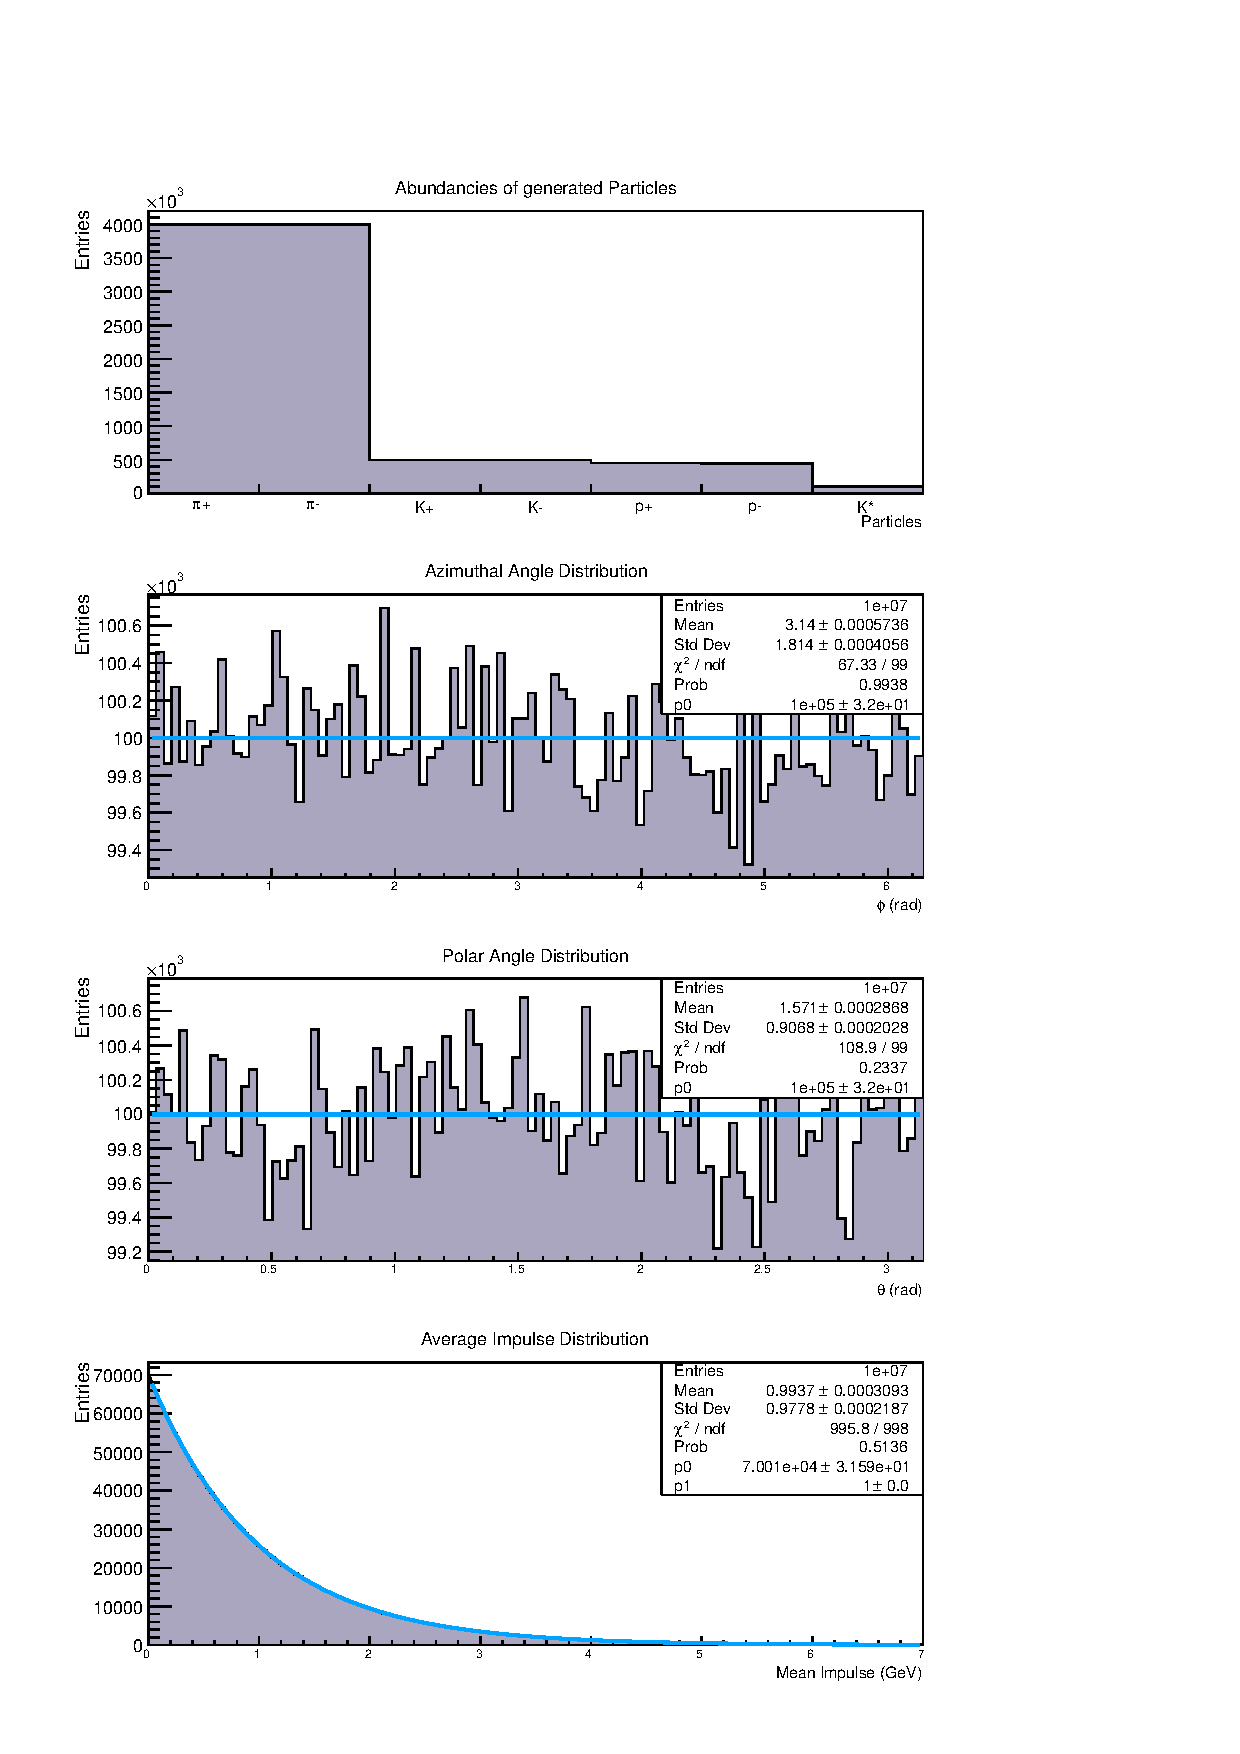
\includegraphics[height = 1.05\textheight]{ParticlesHistos.pdf}
    \caption{Particles}
    \label{fig:Particles}
\end{figure}
\begin{figure}[ht]
    \centering
    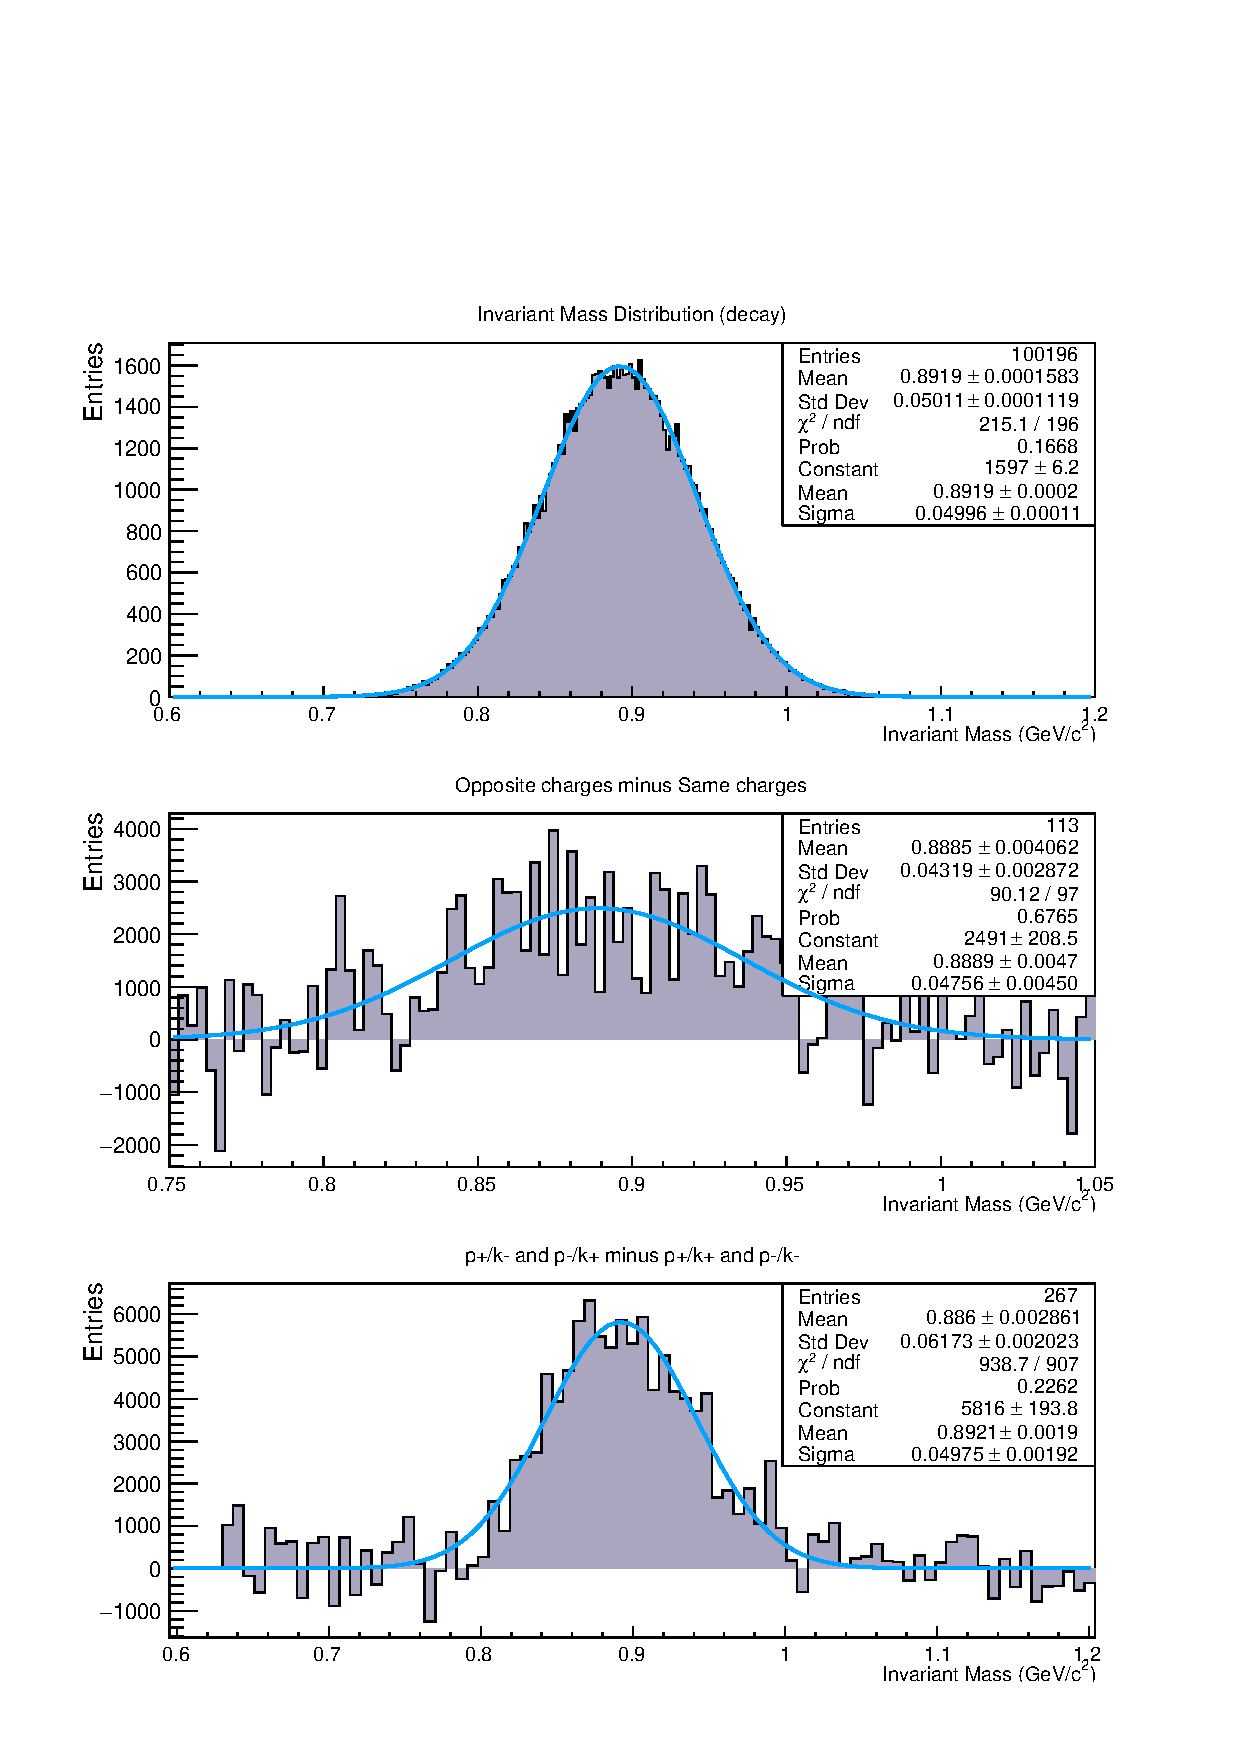
\includegraphics[height = 0.9\textheight]{InvMass.pdf}
    \caption{Invariant mass}
    \label{fig:InvMass}
\end{figure}
\section{Listato del codice}
\label{Listato del codice}
\section{Stampa a schermo dei risultati}
\label{Stampa a schermo dei risultati}

\end{document}
